\chapter{Introduction}
\label{cha:introduction}
\epigraph{How do we get people to understand programming?}{Bret Victor}

Bret Victors opening quote represents the basis for learnable programming \cite{victor_learnable_2012}, whose ideas go back to the early days of Smalltalk \cite{kay_early_1993}.
In his essay \emph{The Early History of Smalltalk}, Alan Kay looks back at the events that led to the creation of Smalltalk.
More importantly, he gives insight into the context of why Smalltalk turned out how it did.
Smalltalk was intended to be a learning environment for children, its strong object orientation was a side-effect of this idea \cite{kay_early_1993}.
It turned out that objects, message passing and compositionality allowed people (not only children) using Smalltalk, to align their ways of thinking with the way their programs were structured.
Applying the conversational lens of programming environments (see Section~\ref{sec:conversational-lens}) to Smalltalk, one could argue that speaking the same language results in a shared mental model between the program and the programmer.
Or as Weinberg \cite{weinberg_psychology_1971} described the status quo (in 1971): "When we talk to our computers, unhappily, we are usually speaking in different tongues."
Unfortunately, not a lot of effort has been put into aligning those tongues over the last 50 years.

Programming environments that foster this style of communication are usually called live programming\cite{aguiar_live_2019, church_liveness_2010} or interactive programming \cite{czaplicki_interactive_2013, mccabe_towards_2023}.
Usually, such systems possess the following properties \cite{burg_1st_2013}:
\begin{description}
    \item[Liveness] They give the programmer immediate feedback, while the program is edited. This feedback can target the program's output, structure, or both.
    \item[Structure] Environments that are aware of a program's structure, understand and preserve this structure. They operate at the level of structure, not on raw text, simplifying program modifications.
    \item[Tangability] Normally, program execution happens behind the scenes and provides little to no capabilities for live inspection. Tangible programming makes a program's execution transparent, tangible, and explorable.
    \item[Concreteness] It is way easier for people to start with concrete examples and generalize later on.
\end{description}

Live programming systems lead to tighter feedback loops.
This outcome was described by \citeauthor{hancock_real-time_2003} \cite{hancock_real-time_2003} and illustrated in \cite{aguiar_live_2019} as shown in Figure~\ref{fig:bow-arrow} and Figure~\ref{fig:waterhose}.
%
\begin{figure}[h]
\centering
\includesvg[width=0.75\textwidth]{images/arrow-bow}
\caption{When trying to hit a target with a bow and arrow, one can only re-aim based on the previous shot. Feedback is provided only after the arrow reaches the target. Image source~\cite{aguiar_live_2019}.}
\label{fig:bow-arrow}
\end{figure}
%
Hitting a target with a bow and arrow vs. hitting it with a hose indicates multiple differences.
The most obvious one is the constant stream of information that is provided by observing where the water hits the target when using a hose.
But is this uninterrupted stream of information really the reason why it is easier to hit a target with a hose?
Hancock \cite{hancock_real-time_2003} argues that this is only a fraction of the reason, according to his interpretation the main difference is that the waterer \emph{never stops aiming}.
While the archer's actions consist of a series of distinct actions (while having to re-aim after each shot), the waterer does not have to "reload".
Hence the waterer does not need to switch contexts, while at the same time being supported by continuous feedback.
One can also visually perceive the shortened feedback loop between Figure~\ref{fig:bow-arrow} and Figure~\ref{fig:waterhose}.

\begin{figure}[h]
\centering
\includesvg[width=0.6\textwidth]{images/waterhose}
\caption{Aiming with a hose is much easier. Continuous feedback allows the person using the hose to constantly re-adapt to the target, without having to stop aiming at all. Image source~\cite{aguiar_live_2019}.}
\label{fig:waterhose}
\end{figure}

In contrast to the previously described problem of speaking the same tongue, several frameworks and programming tools are actively trying to shorten the feedback loop \cite{kubelka_road_2018}.
Web development tools\footnote{\url{https://firefox-dev.tools/}} in major browsers support direct page editing, Vitest\footnote{\url{https://vitest.dev/}}, a testing framework for JavaScript supports an instant watch mode, all modern web frameworks support hot-module replacement\footnote{\url{https://webpack.js.org/concepts/hot-module-replacement/}}, qwik\footnote{\url{https://qwik.builder.io/docs/}} lets developers click at components which takes them directly to the source code. Redux\footnote{\url{https://redux.js.org/}} allows developers to travel through their application state by providing time-traveling debugging.
REPLs are kind of standard for newly developed languages\footnote{\url{http://docs.idris-lang.org/en/latest/reference/repl.html}}, Java and .NET support hot-reloading under certain circumstances\footnote{\url{https://docs.spring.io/spring-boot/docs/2.0.x/reference/html/howto-hotswapping.html}}\textsuperscript{,}\footnote{\url{https://learn.microsoft.com/en-us/visualstudio/debugger/hot-reload}} and Apple's Swift programming language supports live programming with interactive playgrounds\footnote{\url{https://developer.apple.com/swift-playgrounds/}}.
Although this list is by far not exhaustive and there is a clearly visible trend towards live programming, comparing tools used in industry to the properties of live programming, there is still a huge gap.
The next section portrays the concept of interactive programming in the broader context of software development, compared to the text-producing act of programming.

% \todo[inline,color=blue!40]{Maybe cross-reference to Psychology of Programming and explain that faster feedback fosters happiness.}



\section{Context}
\label{sec:context}
Continuing this idea of comparing programming and software development one can observe that programming is just a fraction of the whole software development process \cite{yang_phase_2008}.
A common view on the software development phases is \begin{enumerate*}[label=(\roman*)]
\item planning,
\item requirements analysis,
\item designing,
\item coding,
\item testing,
\item delivery and
\item maintenance
\end{enumerate*},
revealing that programming is indeed mainly part of coding and maintenance.
Although code-driven approaches targeting requirements analysis \cite{sheldon_software_2000}, designing \cite{pimentel_requirements_2014}, testing \cite{beck_test-driven_2003}, and delivery (continuous delivery \cite{chen_continuous_2015}) are becoming more and more popular, creating software is still more than coding.
Successfully applying ideas of live programming to more aspects of the software development process than programming requires a closer look at these processes as well as their history.

% \todo[inline]{This feedback-loop metaphor can be applied to a specific developer, a team or even with customer-interaction.}
% \todo[inline]{In the introduction I did not differentiate between programming and software development, but it is a huge differentiation.}
% \todo[inline]{Explain the differences between psychology of programming and psychology of software development and what it has to do with requirements to code and idea to code.}

\subsection{Agile Software Development}
\label{sec:agile-movement}
The aforementioned feedback loops are applicable to a wide range of problems.
As such, software development or software engineering approaches might be considered.
Viewing their history through the lens of tightening feedback loops provides an additional perspective on why people adopted agile software development practices.

Working on projects, especially in teams, always follows a structure.
In software engineering, this structure is defined by software development methods.
When software engineering came up, practitioners adapted already existing project management methodologies to it, leading to highly rigid methods, in the beginning \cite{misra_agile_2012}.
Those now called \emph{traditional software development methods} were focused on following well-defined plans and detailed documentation.
According to \citeauthor{misra_agile_2012}'s overview of the history of agile software development practices \cite{misra_agile_2012}, these rigid methods worked well for compilers and operating systems, but their heavy focus on well-defined plans was not flexible enough for developing small business applications as well as spreadsheets.
Although, being formalized in 2001 by \citeauthor{beck_manifesto_2001}, the origins of the agile software manifesto's ideas \cite{beck_manifesto_2001} date back to the early software development methods \cite{van_der_aalst_historical_2008}.
The core idea of the agile manifesto is defined as below:
%
\begin{quote}
    We are uncovering better ways of developing software by doing it and helping others do it.
    Through this work we have come to value:
    %
    \begin{itemize}
        \item \emph{Individuals and interactions} over processes and tools.
        \item \emph{Working software} over comprehensive documentation.
        \item \emph{Customer collaboration} over contract negotiation.
        \item \emph{Responding to change} over following a plan.
    \end{itemize}
    %
    That is, while there is value in the items on the right, we value the items on the left more.
\end{quote}
%

Alongside their manifesto, \citeauthor{beck_manifesto_2001} published twelve principles for developing software in an agile way.
Table~\ref{tab:agile-principles} lists these principles.
Based on the agile manifesto and the ideas of interactive programming, each of the principles is interpreted in how it might align with the fundamental idea of tightening the feedback loop.
If applicable, the interpretation also draws comparisons to how interactive programming might be beneficial for this specific principle.

\begin{block}
\begin{ThreePartTable}
\begin{TableNotes}
\footnotesize
\item \textit{Note:} The character "---" denotes that applying the lens of tightening the feedback loop through live programming does not yield any meaningful results.
\end{TableNotes}
%\setlength{\tabcolsep}{10pt}     % separator between columns (standard = 6pt)
%\renewcommand{\arraystretch}{1.50} % vertical stretch factor (standard = 1.0)
%\caption{Applying the lens of tightening feedback loops through live programming to the agile principles \cite{beck_manifesto_2001}.}
%\label{tab:agile-principles}
%\centering
%\newcommand{\RR}{\rightskip=0pt plus1em \spaceskip=.3333em \xspaceskip=.5em\relax}
\renewcommand{\arraystretch}{1.30}
\small
%    \begin{english}
%    \begin{tabular}{@{}p{0.4\textwidth}p{0.55\textwidth}}
\begin{longtable}{@{}cp{0.35\textwidth}p{0.5\textwidth}@{}}
    % -------------------------- first header ----------------------------
    \caption{Applying the lens of tightening feedback loops through live programming to the agile principles \cite{beck_manifesto_2001}.} 
    \label{tab:agile-principles}																						 \\
    \toprule
    \# & Agile Principle & Interpretation \\
    \midrule
    \endfirsthead
    % ---------------------- subsequent headers ---------------------------
    \caption*{\textbf{Table \getcurrentlabel} (\emph{continued})}				 \\
    \toprule
    \# & Agile Principle & Interpretation \\
    \midrule
    \endhead
    % --------------------------------------------------------------------
    \toprule
    \# & Agile Principle & Interpretation \\
    \midrule
    \endhead
    
    \insertTableNotes  % tell LaTeX where to insert the contents of "TableNotes"
    \endlastfoot
    
    (1) &
    Highest priority is given to satisfying the customer through early and continuous delivery of valuable software. &
    This principle provides evidence for tightening the feedback loop between the customer and development team.
    Continuously delivering software gives the customer the feeling of "being in the loop".
    \\
    (2) &
    Changing requirements are welcome, even late in development. Agile processes harness change for the customer’s competitive advantage. &
    According to \cite{van_der_aalst_historical_2008}, customers might not know their full problem space.
    Iterating on potential solutions, while close communication between development teams and customers is emphasized, leads to a co-exploration of the problem, as well as the solution space, enabled by tighter feedback loops.
    \\
    (3) &
    Working software is delivered frequently, from a couple of weeks to a couple of months, with a preference to the shorter timescale. &
    A perfect example for tightening the feedback loop between different versions of software.
    One should note the emphasis on "with a preference to the shorter timescale" which actively promotes shorter feedback loops.
    \\
    (4) &
    Business people and developers work together daily throughout the project. &
    Working together on a daily basis actively reduces the amount of documentation overhead, hence it shortens feedback loops.
    However one has to be aware of the side effects imposed by this (see \ref{sec:programming-as-theory-building} for an alternative take on the topic of documentation in software projects).
    \\
    (5) &
    Projects are built around motivated individuals.
    They are given the environment and support they need, and trusted to get the job done. &
    ---
    \\
    (6) &
    It is believed that the most efficient and effective method of conveying information to and within a development team is face-to-face conversation. &
    Again, face-to-face conversation is as short as a feedback loop can get.
    Applying interactive programming in a way that fosters face-to-face conversation about certain solutions would enhance this even more.
    \\
    (7) &
    It is believed that working software is the primary measure of progress.&
    ---
    \\
    (8) &
    It is believed that agile processes promote sustainable development.
    The sponsors, developers, and users should be able to maintain a constant pace indefinitely.&
    ---
    \\
    (9) &
    It is believed that continuous attention to technical excellence and good design enhances agility.&
    ---
    \\
    (10) &
    It is believed that simplicity – the art of maximizing the amount of work not done – is essential.&
    This principle can be approached in at least two ways.
    First, "maximizing the amount of work not done" could be applied to feedback loops in a way that no need for a feedback loop is even faster than a very tight one.
    Secondly, certain ideas of live programming could be utilized to prevent unnecessary features from being developed, thus contributing to simplicity.
    \\
    (11) &
    It is believed that the best architectures, requirements, and designs emerge from self-organizing teams.&
    The advantage of self-organizing teams could be caused by tighter feedback loops, leading to less feedback that gets mis-transferred.
    \\
    (12)&
    It is believed that success is achieved when at regular intervals the team reflects on how to become more effective, then tunes and adjusts its behavior accordingly.&
    Retrospectives perfectly showcase what happens when tighter feedback loops (in this case about the internal team dynamics) are applied to software development.
    \\
    \bottomrule
\end{longtable}
\end{ThreePartTable}
\end{block}

Summing up those principles, agile software development encourages lean development using iterative and evolutionary approaches.
Close collaboration between software development and business teams should lead to higher customer satisfaction by actually incorporating their (possibly changing) needs, instead of emphasizing processes and documentation.
Face-to-face communication, frequent deliveries, adapting and properly managing changing requirements, as well as having organizational capabilities which enable this, are necessary premises for implementing agile software development processes successfully \cite{misra_agile_2012}.
These original ideas were more and more commercialized with various frameworks being created based on the agile philosophy \cite{hohl_back_2018}.
According to \citeauthor{hohl_back_2018}, Scrum is often seen as the only agile practice.
Because managers and developers mainly apply frameworks, the initial diversity as well as the underlying principles of the agile manifesto get lost.


%\todo[inline]{somehow incorporate: Therefore, it is important for the business, and the development teams to work hand-in-hand throughout the entire duration of the project.}

Interestingly, already the waterfall method \cite{royce_managing_1987}, classified as a traditional software development method, defines feedback loops between successive stages of the software engineering process.
It also introduced the stage of prototyping, intended for improving the phase of requirements analysis and design as early as possible.
Combining these feedback loops with the core idea of the spiral model \cite{boehm_spiral_1988}, which introduces the idea of an iterative approach in contrast to sequentially approaching the phases of software development, reveals the origins of agile practices \cite{misra_agile_2012}.
In the next section, we are gonna take a brief look at the topic of prototyping and how agile ideas have been applied to different types of prototyping.


\subsection{Prototyping}
In his essay \citetitle{gladden_stop_1982} about the shortcomings of the waterfall model, \citeauthor{gladden_stop_1982} argues that sequential software development processes lead to missed schedules and the creation of unsuccessful products in a sense that the produced software \begin{enumerate*}[label=(\roman*)]
\item does not perform the function intended, or
\item does not satisfy the customer's needs
\end{enumerate*}
and calls for a different form of collaboration between the involved parties \cite{gladden_stop_1982}.
His argumentation consists of the inherent complexity of communicating requirements between different parties, the huge impact of changing requirements and the elapsed time between specifying requirements and actually seeing their outcome.
Introducing the \emph{Non-Cyclical (Hollywood) Model}, he proposes that: "Nothing conveys more meaning or serves to congeal a system concept better than the system itself" \cite{gladden_stop_1982}.
Instead of defining (textual) requirements, customers should present their objectives and work together with the development team on agreeing upon them.
One of his described techniques for achieving objectives is \emph{rapid prototyping}.
For properly understanding prototyping it might make sense to take a look at the etymological origin of said word: \emph{prototype} is analyzable as \texttt{proto-} and \texttt{type}.
The word's origin goes back to Ancient Greek \emph{\textgreek{πρωτότυπος}} (original; prototype), with the conjunction of \emph{\textgreek{πρῶτος}}, (first; earliest) and \emph{\textgreek{τῠπος}} (pressing; sort; type). % ῠ́π

This is mainly how the concept of a prototype is understood in software development \cite{budde_what_1992}, with slight differences in interpretation.
Although these interpretation differences are not big, their effects do not really align with the original concept of a prototype.
We will refer back to the etymological origin of the word \emph{prototype} to depict some of those contradictions.

Prototypes are used to create a shared understanding between developers, users, and management \cite{budde_what_1992}.
They are used to identify difficulties, clarify problems and misunderstandings, and help in making design decisions.
If necessary, they are complemented with written system specifications.
According to \cite{budde_what_1992} a prototype that "is used for more than [the] experimental testing of an idea for illustrative purposes, but rather is employed in the core of the application" is known as a \emph{pilot system}.
A pilot system requires a much more elaborate design than a prototype.
Applying the etymological perspective, a "first type" of some program does not have to be as stable or as mature as if it is part of the finished product.
Although \citeauthor{budde_what_1992} clearly distinguish prototypes from pilot systems, this looks very different in practice.
They already present this contradiction in their article when explaining different goals of prototyping \cite{budde_what_1992}.
\begin{enumerate*}[label=(\roman*)]
\item \emph{Exploratory Prototyping} is used when the problem to solve is unclear or underspecified. In this case, prototyping is used to evaluate different solutions and clarify requirements.
\item \emph{Experimental Prototyping} can be seen as a technical feasibility study. Developers experiment with the help of prototypes to find out whether existing requirements can be fulfilled.
\item \emph{Evolutionary Prototyping} emphasizes the nominalized verb \emph{prototyping} over the noun \emph{prototype}. The focus lies on the process of creating one prototype after another, leading to prototypes being converted to pilot systems, being converted to the actual product. This interpretation contradicts the ancient Greek understanding of the word prototype. Visualizing processes involving the progress of time is easier when shown graphically, thus Figure~\ref{fig:throw-away-prototyping} and Figure~\ref{fig:evolutionary-prototyping} show these differences.
\end{enumerate*}

Matching the meaning of the word prototype, throw-away prototyping (as shown in Figure~\ref{fig:throw-away-prototyping}) treats prototypes as artifacts from ideation phases.
The source code of these prototypes is \emph{not} reused later when the application itself is developed.
Knowing that the source code will not be reused creates a mindset where software engineers focus on creating the functionality that should be prototyped and do not focus on code style and maintainability.
Sketching and prototyping are usually two different things.
Sketching is focused on the user interface and user experience and does not concern the technical implementation of a piece of software.
The phases (depicted as arrows) in Figure~\ref{fig:throw-away-prototyping} highlight that developing features starts after their respective sketching or prototyping phases.
%
\begin{figure}
    \centering
    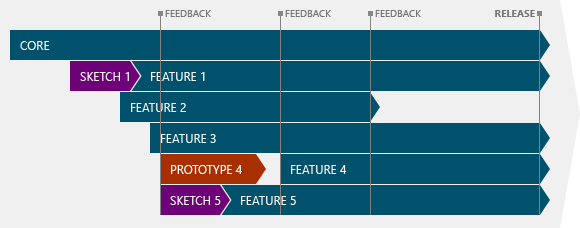
\includegraphics[width=0.8\textwidth]{images/throw-away-prototyping}
    \caption{Throw-away prototyping and sketching: prototypes help gather early feedback before starting to develop the actual feature. Image source~\cite{mourzenko_why_2014}.}
    \label{fig:throw-away-prototyping}
\end{figure}
%
In contrast to throw-away prototyping, the concept of evolutionary prototyping (as shown in Figure~\ref{fig:evolutionary-prototyping}) incorporates customer feedback iteratively and incrementally over the whole process of product development.
As described in \cite{mourzenko_why_2014}, code style, maintainability, design patterns, and testing count from the beginning of development, because starting with an early prototype the actual product is an evolution of it.
As depicted in Figure~\ref{fig:evolutionary-prototyping}, based on feedback and requirements new features are added as well as existing ones are adapted or removed, leading to the final product.
This evolutionary approach clearly contradicts the original definition of prototype being a \emph{first type}.
Furthermore, if a project is started with the premise of developing a prototype, developers should write code that adheres to the philosophy of prototyping, which intentionally excludes proper code style as well as software architecture.
If such a prototype should then be evolved into an evolutionary one, this basis is missing, making it exponentially harder to properly introduce a solid, scalable architecture that supports the requirements of a long-living product.
%
\begin{figure}
    \centering
    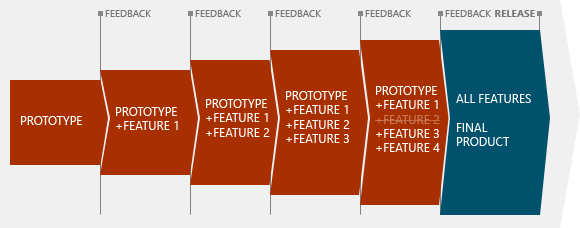
\includegraphics[width=0.8\textwidth]{images/evolutionary-prototyping}
    \caption{Evolutionary prototyping: features are aggregated to the prototype to build the final product. Image source~\cite{mourzenko_why_2014}.}
    \label{fig:evolutionary-prototyping}
\end{figure}

\subsubsection{Wizard of Oz Prototyping}
\label{subsub:wizard-of-oz-prototyping}
One other interesting type of prototyping for the context of this thesis is \emph{Wizard of Oz Prototyping} \cite{dow_wizard_2005}.
The Wizard of Oz Methodology has its origins in human-computer interaction research, specifically in the area of "exploring user interfaces for pervasive, ubiquitous,
or mixed-reality systems that combine complex sensing and intelligent control logic" \cite{dow_wizard_2005}.
It would take an immense amount of resources to create such an interface, but if one is able to draw a sensible line between the user interface and its actual implementation, this implementation can be simulated by humans.
This enables the system to be tested, without the need for it to be implemented, which again aligns with the original meaning of the word prototype.
The etymological origin of the Wizard of Oz methodology can be traced back to the "American children's book \emph{The Wonderful Wizard of Oz} by Frank Baum, in which the characters meet a giant head, that appears to be a powerful wizard, only to learn that it’s just an ordinary man pulling levers behind a screen" \cite{ramaswamy_wizard_2022}.

%\todo[inline,color=blue!40]{Maybe look into Rapid Application Development and its approach on Prototyping}
%\todo[inline]{Bring the concept of tactical programming vs. strategic programming into play (based on Osterhout as described in my Psychology BA)}
%\todo[inline]{Mention that prototypes get released to production (Tesla, Spotify, Apple) and that customers do the testing.}
%\todo[inline,color=blue!40]{Maybe bring in a little bit of capitalism criticism in the form of market fit vs. high-quality products, just show the contradiction.}


%\subsection[Interactive Programming]{Interactive Programming \protect{\estimatedpagecount{.5}}}
%\todo[inline]{Bridge the gap between prototyping and interactive/live programming as described in the introduction. Mention how this might align with agile methodologies, the psychology of programming and customer-centered approaches.}


\section{Problem Statement}
As stated in \citetitle{anonymous_what_1967}, programming is primarily a communication process \cite{anonymous_what_1967}.
Even if programming is not seen as a mainly human-centered activity, translating thoughts into a language understood by machines is a form of communication, namely \emph{Human Computer Interaction} (HCI) \cite{myers_past_2009}.
As already described in Section~\ref{sec:context} analyzing the broader context of programming, namely software development emphasizes the relevance of communication as well.
Whether they are called requirements or objects, the users' needs have to be identified and translated into working code.
Agile development practices foster the creation of successful applications by bringing stakeholders together and allowing them to iterate on proposed solutions.
Prototyping is one such tool that enables the co-creation of software, but if it is applied incorrectly (oftentimes because of tight schedules) it leads to brittle and unstable products.
Live-Programming can also be interpreted as a tool to enable the co-creation of software, but it is mainly aimed at helping a specific developer understand how and why some code works.
One could argue now, that programming tools (frameworks, environments, languages, ...) are not optimized for the agile co-creation of software while still emphasizing technical scalability and longevity.
This section is aimed at clarifying this problem statement, as well as providing deeper insights into the social as well as psychological characteristics of developing software.

%As stated in \textcite{curtis_psychology_1990} mainly organizational processes characterize software development.

\subsection{Programming as Complex Problem Solving}
Complex problem solving is a research discipline in psychology that is concerned with how humans solve complex problems.
There are a lot of arguments about the definition of \emph{a complex problem}, with an overview presented in \cite{dorner_complex_2017}.
As defined by \citeauthor{funke_complex_2012}, a complex problem is defined by
\begin{enumerate*}[label=(\roman*)]
\item its immense amount of involved variables,
\item a lot of dependencies between those variables,
\item the dynamics of the situation
\item (partial) intransparency of those variables and their connections, and
\item \emph{polytely} (the Greek term for “many goals”), resulting in goal conflicts \cite{funke_complex_2012}.
\end{enumerate*}
Complex problems can further be divided into the categories \emph{well-defined} and \emph{ill-defined}.
Well-defined problems do have a fixed problem space as well as a fixed solution space.
Their problem state and goal state are both well-known.
An example of a well-defined problem is the assignment to write a program that prints some text $n$ times.
As a solution one could either copy and paste the print statement $n$ times or create a loop that prints said text $n$ times.
Ill-defined problems do not have a clear problem definition, a desired goal and there is no obvious and clear way of reaching the goal.
Most programming problems that are more complex than printing some text $n$ times are ill-defined problems.
It becomes even more clear, if one takes a more holistic view of software development, compared to "just" programming.
Usually, a group of people has to create some product that fits some needs, resulting in a partially open problem as well as solution space with many potential ways of getting there.

Multiple studies have been conducted on the programming part of complex problem solving \cite{lawan_what_2019, gibson_software_2005, robertson_role_2008, taheri_evaluating_2015}, whereas the research area of complex problem solving applied to actual software development was researched quite sparsely \cite{wingo_using_2015}.
\citeauthor{curtis_psychology_1990} pointed this out as early as 1990 \cite{curtis_psychology_1990}: "The fact that this field is usually referred to as the `psychology of programming' rather than the `psychology of software development' reflects its primary orientation to the coding phenomena."
This research problem gets multiplied by the fact that conducting experimental research regarding complex problem solving is hard to closely align to reality.
Although a lot of variables can be introduced as well as controlled in a lab situation, complex problems are also defined by the dynamics of their situation, complicating experimental designs and making their results less applicable to real-world scenarios \cite{lawan_what_2019}.


\subsubsection{Top-Down vs. Bottom-Up}
Top-down and bottom-up are both methods to approach problems.
Both approaches describe how to handle the decomposition as well as the composition of sub-problems.
Especially the before mentioned \emph{complex problems} need strategies for solving them.

If a problem is defined quite openly and broadly, applying the top-down approach proved to be fitting \cite{kung_comparing_2013}.

As described by \citeauthor{kung_comparing_2013} \cite{kung_comparing_2013}, "Adoption of a top-down approach will generally start with a set of high-level requirements, such as a narrative."
Thus, problems that benefit from approaching them in a top-down manner, do usually have an open and broad problem definition, hence their problem as well as their solution scope still need to be explored.
Figure~\ref{fig:top-down} depicts a visual representation of the top-down approach showing how the problem and solution space are explored starting from the top.
The more \emph{ill-defined} a problem presents itself, the better the top-down approach works.
%
\begin{figure}[h]
\centering
\hspace*{0.15\linewidth}
\includesvg[width=0.75\textwidth]{images/top-down}
\caption{Approaching a problem in a top-down way. The intensity of a rectangle's color conveys information about how well the (sub-)problem and solution space are already explored. Exploring the problem starts at the top and it is divided into smaller sub-problems.}
\label{fig:top-down}
\end{figure}
%
The opposite approach is depicted in Figure~\ref{fig:bottom-up}.
One needs to already know what the "bottom" of the problem under investigation is to apply the bottom-up method successfully.
As described by \citeauthor{jones_is_2011} \cite{jones_is_2011}: "To use the bottom-up method you need to be able to efficiently determine what the `bottom' is, which usually means you need a heavily constrained problem space."
Already existing partial solutions are composed in such a way that they solve the full problem.
Well-defined problems can usually be solved quite well using the bottom-up method because if the problem space is well known and solutions for these sub-problems exist, they "just" need to be assembled.
%
\begin{figure}
\centering
\hspace*{0.15\linewidth}
\includesvg[width=0.75\textwidth]{images/bottom-up}
\caption{Approaching a problem in a bottom-up way. The intensity of a rectangle's color conveys information about how well the (sub-)problem and solution space are already explored. Solving the problem starts at the bottom, where already existing solutions are composed together so that the whole problem can be solved.}
\label{fig:bottom-up}
\end{figure}
%
Although we just introduced a clear distinction between top-down and bottom-up approaches, in reality (regarding programming as well as software engineering) a combination of both is used.
Requirements are rarely so clear that developers immediately know how to approach them bottom-up, but existing solutions for cross-functional requirements like logging or authentication might be well known and can be applied directly.
This leads to a mixture of top-down and bottom-up usage, where parts of the solution have to be explored with a general concept in mind, whereas other parts of the problem can already be solved with existing solutions.
Applying this insight to programming imposes the interesting question of how to combine both approaches to keep track of what is already solved and what is not.
Keeping track of something can be seen as an act of conversation, \citeauthor{mccabe_towards_2023} applied this lens to modern development environments, the next chapter sums up his ideas and explains the motivation behind them.


\subsubsection{Conversational Lens regarding Complex Problem Solving in Development}
\label{sec:conversational-lens}
Modern development environments and analysis tools point out various possible bugs and vulnerabilities based on static code analysis.
As research has shown, those results are commonly not respected \cite{mccabe_towards_2023}.
Alan T. McCabe has analyzed why they are not used as much as they could be, with the most prominent reasons being:
\begin{enumerate*}[label=(\roman*)]
\item false-positives, leading to a lot of noise;
\item poor understandability, causing frustration and non-motivation to dig into these reports; and
\item a lack of integration into the developer's workflow, forcing developers to switch contexts and drop out of being in the flow.
\end{enumerate*}
Based on these discoveries \citeauthor{mccabe_towards_2023} et al. approached the improvement of development tools through the conversational lens.
Drawing from observations around the mechanics of human conversations, they try to apply human-like conversation approaches to the code analysis tools.
However, it is of high importance, that they do not want to anthropomorphize those tools, rather they want to align interactions in such a way that more accurate mental models can be built.
By targeting the observability of compilation processes and "framing an interaction as a `conversation' between a human and their development environment" \cite{mccabe_towards_2023} the compiler's \emph{thought process} can be externalized and understood by the developer in a similar way as misunderstandings can be clarified when when talking with another human being.

Edwin Brady shares a similar view on compilers, he imagines the compiler as the "lab assistant", in a way that the compiler should take part in a pair programming exercise, helping developers accomplish their goals.
An example of how this works is shown in Section~\ref{sec:introducing-hole-driven-development}.


\subsubsection{Programming as Theory Building}
\label{sec:programming-as-theory-building}
Applying the conversational lens to the greater context of developing software in teams and organizations leads to Peter Naur's influential paper \citetitle{naur_programming_1985}.
Bridging the gap between the psychology of programming and the psychology of software development, the findings of this paper constitute a major part of this thesis hypothesis, hence there is a separate section dedicated to it.

Peter Naur argues that programming is not an activity of mere text production, rather it is an activity of creating a shared understanding while the activity of text production itself should be understood as a series of program modifications.
He highlights the importance of a correct understanding of programming like the following: "If our understanding is inappropriate, we will misunderstand the difficulties that arise in the activity and our attempts to overcome them will give rise to conflicts and frustrations. \cite{naur_programming_1985}"
After clarifying that he uses the term \emph{programming} to denote the whole activity of design and implementation (at the beginning of Chapter~\ref{cha:introduction} we differentiated between \emph{programming} and \emph{software development} with the latter one being synonymous to Naur's understanding) he introduces his Theory Building View based on Ryle's definition of the word \emph{theory} \cite{ryle_concept_1984}.
The possession of a theory is not defined by any particular knowledge of facts, but by being able to do things, accompanied by explanations, justifications, and responses to queries about it \cite{barn_revisiting_2011}.

Building upon this definition, Naur continues to argue that to bring new programmers onto a team, they have to work in close contact with programmers who already possess the theory.
Because there is no particular sequence of actions (method) that is underlying the process of theory building, theories cannot be documented via textual artifacts.
With the essence of the program, its theory, being inextricably bound to human beings, the role of programmers changes from one that produces source code and documentation (an easily replaceable one) to one that possesses the vital theory about those artifacts.
Based on these insights Naur argues that the assumption that software is easy and cheap to modify is a fallacy.
Because it is not the source code of a program that has to be modified, but rather the theory (shared understanding) modification of software is e.g. comparable to the modification of buildings, which is known to be expensive and in fact, sometimes it is economically preferable to demolish the existing building and re-build it as a whole.
Arguing that creating highly flexible programs diminishes the need for modification is the next fallacy, because the increase in complexity introduced by flexibility leads to substantial costs already upfront.
According to Naur, because programming is an act of theory building, we should emphasize ways of improving the sharing of understanding, hence the formation of theories.

\subsubsection{Applying Philosophy to the Theory Building View}

In their contemporary philosophical analysis of agile software development, \citeauthor{northover_agile_2007} applied Karl Popper's philosophy of \emph{evolutionary epistemology} to software development \cite{northover_agile_2007}.
According to Popper \cite{northover_karl_2006}, all advances in knowledge follow the following model:

\[P_1 \rightarrow TS \rightarrow EE \rightarrow P_2\]

$P_1$ is the initial problem, $TS$ is the proposed solution, $EE$ is the process of error elimination applied to $TS$, and $T_2$ the resulting solution containing new problems \cite{northover_karl_2006}.
Applying this model to the context of iterative software development, \citeauthor{northover_agile_2007} interpret it as the following: $P_1$ is the initially identified subset of requirements, $TS$ corresponds to the solution proposed by the developer -- "the developer's `theory'" \cite{northover_agile_2007}, $EE$ are the testers' attempts on eliminating errors by creating test cases and $P_2$ corresponds to a tested subset of the software.

With Naur's Theory Building view in mind, one could argue that by interpreting the model in the way \citeauthor{northover_agile_2007} did, such that developers are not included in the $EE$ stage, hardly allows them to improve their theory of the system.
Only by including them in the error elimination phase ($EE$) enables them to refine and adapt their theories of the system.
This interpretation is continued in \ref{sec:hypothesis}.


\subsection{Cognitive Load}
\label{sec:cognitive-load}
The term \emph{cognitive load} is used in cognitive psychology to describe the amount of working memory that has to be used by a person while performing a task \cite{shaw_memory_2016}.
The human memory is divided into working memory (sometimes also called short-term memory) and long-term memory.
Their capacity is on an entirely different scale \cite{seemann_code_2021} with the short-term memory being able to store around four to seven items \cite{shaw_memory_2016}.
Applying a reductionistic machinistic view of humans one can compare this to a computer's memory and storage model.
Working memory can be accessed incredibly fast, but has a limited storage capacity, while permanent storage is slower, but it can store a magnitude of information that can be held in memory.

Applying this knowledge to the act of developing software highlights some of its problems.
Efficiently writing software demands a lot of information to be kept in memory, but firstly our brains aren't made for keeping track of many things at the same time and secondly, we tend to skip doing things that aren't of high importance at the moment.
As put into words by Mark Seemann \cite{seemann_code_2021}: "The problem isn't that you don't know how to do a thing; it's that you forget to do it, even though you know that you ought to."
Empirical studies conducted in the field of resource theories \cite{ormerod_human_1990} have shown that during programming, performance is limited because attentional and memory resources have to be divided up amongst competing processes.
It has been shown that this resource limitation is responsible for programming errors, thus suggesting that these errors could be reduced by decreasing the need for working memory, resulting in lower cognitive load \cite{ormerod_human_1990}.

Programming is by far not the only discipline where a lack of working memory influences performance.
Pilots and surgeons use checklists so that they don't forget tasks that might end up being lethal \cite{seemann_code_2021}.
Another method of reducing cognitive load can be achieved using 3M's Post-Its™.
Empirical studies \cite{digiano_learning_nodate, dove_grouping_2018} have shown that Post-Its™, perfectly fit collaborative activities, because of them
\begin{enumerate*}[label=(\roman*)]
\item being of limited size, leading to them capturing one single thought;
\item being re-arrangeable and re-groupable, which conveys meaning;
\item being physically unique, which suggests turn-taking in editing or changing via natural affordances;
\item and them being ephemeral, which reduces the cognitive bias of effort justification \cite{norton_ikea_2012}, leading to the Post-Its™ being discarded if no longer needed
\end{enumerate*}.

Applying these ideas back to programming, as any non-trivial software being of such a size that is not graspable by working memory alone, its code structure needs to be decomposable and compartmentizable so that these chunks can fit in the programmer's brains.
Or as Kent Beck puts it\footnote{\url{https://twitter.com/KentBeck/status/1354418068869398538}}: "The goal of software design is to create chunks or slices that fit into a human mind. The software keeps growing, but the human mind maxes out, so we have to keep chunking and slicing differently if we want to keep making changes."



\section{Tackling Complexity}
\label{sec:tackling-complexity}
After presenting some challenges of how complexity affects software development, this section introduces two concepts how complexity can be managed and how cognitive load can be reduced.


\subsection{About Todo-Comments}
\label{sec:introduction-about-todo-comments}
Comments are informal parts of source code that do not get executed, they often make up for a considerable amount of a program's source code \cite{nie_natural_2018}.
If those comments are prefixed with \emph{TODO} or something alike (e.g. \emph{FIXME}, \emph{UNDONE}, \emph{HACK} or \emph{XXX} \cite{storey_how_2009}), they are considered as todo-comments \cite{ying_source_2005}.
Such a prefix changes their meaning as Robert C. Martin explains \cite[p. 59]{martin_clean_2009}:
%
\begin{quote}
    TODOs are jobs that the programmer thinks should be done, but for some reason can't do at the moment. It might be a reminder to delete a deprecated feature or a plea for someone else to look at a problem. It might be a request for someone else to think of a better name or a reminder to make a change that is dependent on a planned event. Whatever else a TODO might be, it is not an excuse to leave bad code in the system.
\end{quote}
%
A quick analysis based on the search term "todo comments" on the Q\&A-platforms StackOverflow\footnote{\url{https://stackoverflow.com/}} and StackExchange (Software Engineering)\footnote{\url{https://softwareengineering.stackexchange.com/}} lead to $645$ discussion entries ($500$ for the former and $145$ for the latter, query date: 2023/11/01) regarding the topic of todo-comments, indicating an extensively discussed topic.

This might also be based on the fact that in contrast to the formal parts of the source code, comments (hence todo-comments as well) represent the informal part about source code \cite{ying_source_2005, nie_framework_2019, sridhara_automatically_2016, storey_todo_2008}.
Knowledge about them can be shared across different programming languages because apart from the difference in characters indicating comments they do not really differ.
This informal nature imposes challenges for software engineering tools like refactorings or static analyzers but allows programmers to use them in various ways.
They are used for many purposes other than describing code, such as a tool for communication in teams \cite{ying_source_2005}, as bookmarks \cite{storey_how_2009}, for denoting pending tasks \cite{sridhara_automatically_2016} or recording which tests have yet to be defined \cite{storey_todo_2008}.
This makes them extremely versatile and fits Don Knuth's literate programming idea \cite{knuth_literate_1984}, in which he suggests that "programs should not only be intended to be executed by computers but also intended to be read by human \cite{ying_source_2005}."
As promising as this idea sounds, the comments' lack of formality, resulting in a lack of tooling support, leads to them becoming obsolete or "rotting away".
Analyzing the most popular answers of aforementioned quick analysis \cite{karacic_todo_2015, snoop_does_2016, tackabury_how_2019, alecxe_how_2018, squires_use_2012} and combining them with existing empirical \cite{ying_source_2005, nie_framework_2019, storey_how_2009} research led to the following insights about todo-comments:

\subsubsection{IDE Support}
Proper IDE support is necessary for the effective use of todo-comments.
Certain IDEs (e.g. Visual Studio, Eclipse, JetBrains) provide specific views, where todo-comments are aggregated and can be filtered and searched \cite{storey_how_2009}.
Text editors like vim highlight todo-comments visually, resulting in visual code smells.
Regarding the question "Do TODO comments make sense?" one developer answered \cite{karacic_todo_2015}: "Yep, given a listing in your IDE, they are helpful. I would say they're of very limited use otherwise, since the codebase may be enormous."
It is important to note that those features are IDE specific, have to be implemented for each of them, and do not work in online version control systems like GitHub or BitBucket, thus limiting the readability of code.
Without IDE support developers report that it is important to use consistent prefixes for todo-comments, so they can be found via plain text search \cite{karacic_todo_2015}.

\subsubsection{Metadata}
Developers are debating whether it is good or bad practice to include tags (e.g. the author's initials or the todo's creation date) in the comment \cite{karacic_todo_2015}.
Information about a todo's author or its creation date could also be extracted from version control, thus eliminating potential ambiguities.
If a todo-comment targets a specific issue, they should be linked together via the issue number.
\citeauthor{elliott_pep_2005} tried to introduce a standard for tagging todo-comments in Python \cite{elliott_pep_2005}, but the proposal has been dismissed because of no intention to follow this standard in Python's standard library.

\subsubsection{Test-Driven Development}
Developers, following the idea of Test-Driven Development, argue that one should simply write a failing test case, rather than writing todo-comments \cite{snoop_does_2016}.
This might work for well-defined problems and certain cases of todo-comments, but the explorative and versatile nature of todo-comments includes many other use cases than describing missing or invalid functionality.

\subsubsection{Static Code Analysis}
Regarding the adoption, developers argue that: "The main factor is whether or not the team is disciplined enough to follow up on these `little' comments. [...] \cite{karacic_todo_2015}"
Other developers argue that this discipline can be enforced by using static code analysis tools to detect the usage of todo-comments and prevent them from being merged into the main or release branches \cite{alecxe_how_2018}.
These static analysis tools could also be configured in a way that allows todo-comments if and only if they refer to an issue number.

\subsubsection{Creative Usage/Alternatives}
Developers have come up with quite creative solutions to some of the problems mentioned regarding todo-comments.
The .NET standard library includes the class \texttt{\seqsplit{NotImplementedException}}, resembling an exception, that as the name indicates, should be thrown when a method's implementation is missing.
Developers report that they are using this together with todo-comments \cite{squires_use_2012} so that
\begin{enumerate*}[label=(\roman*)]
\item the line of code surfaces in the IDE (because of the todo-comment)
\item and surfaces at runtime (because an exception is thrown)
\end{enumerate*}.
ReSharper\footnote{\url{https://www.jetbrains.com/resharper/}}, an extension for Visual Studio automatically reports usages of \texttt{\seqsplit{NotImplementedException}} in the IDE, preventing developers from having to duplicate things.

Another option for tagging a certain line of code to come back to it after an interruption is to introduce some breaking code, which gets surfaced by the compiler \cite{tackabury_how_2019}.
A quick and easy solution, that unfortunately only works in compiled languages.
One of the most creative ways of surfacing todo-comments at runtime was provided by Drew Hall \cite{tackabury_how_2019}, who created a \CC macro "that expands into constructing a static object at local scope whose constructor outputs a log message".
Using this approach, he is still able use the plain text search based on the macro's name and gets the log messages while running the incomplete program, however the IDE does not report the usage of this macro.



\subsection{Introducing Hole-Driven Development}
\label{sec:introducing-hole-driven-development}
The term \emph{Hole-Driven Development} is not yet scientifically defined, but based on other programming concepts like \emph{Type-Driven Development} \cite{brady_type-driven_2017} or \emph{Test-Driven Development} \cite{mccracken_digital_1957}.
The main idea stems from the \emph{Agda} programming language where \emph{holes} are called \emph{goals}.
Apart from Agda, other languages such as Haskell and Idris feature the concept of holes.
The common properties of those languages is that they are functional, statically typed and therefore have a very sophisticated type system.
These two aspects lay the foundation for Hole-Driven Development as currently understood.

Simply said, a hole declares a missing part in an application.
One can imagine the holes as the blanks in a fill-in-the-blanks exercise.
By deliberately omitting certain expressions in programs, more information about these expressions can be provided by the compiler, which can aid the programmer in properly filling them in.
The example in Listing~\ref{fig:idris-program-hole} was created by \citeauthor{brady_type-driven_2017} for his dependently typed functional programming language Idris \cite{brady_type-driven_2017}.
Idris supports the concept of holes by prefixing expressions with the question mark character (\texttt{?}), which turns these expressions into holes.
In Line~\verb|2| of Listing~\ref{fig:idris-program-hole} the function \verb|main| is defined that should print something (using the standard library function \verb|putStrLn|) to the console.
The hole part of this program is \verb|?greeting| at Line~\verb|2|.
The syntax using a question mark can be understood as formulating a question to the compiler.

\begin{program}
\begin{GenericCode}
main : IO ()
main = putStrLn ?greeting
\end{GenericCode}
\caption{Hole-Driven Development in Idris}
\label{fig:idris-program-hole}
\end{program}

When trying to evaluate the program depicted in Listing~\ref{fig:idris-program-hole}, the Idris compiler will list all holes, as shown in Listing~\ref{fig:idris-compiler-holes}, in this case \texttt{Main.greeting} is shown at Line~\verb|2|.
For interacting with the compiler in this way, Edwin Brady coined the phrase "the compiler as your lab assistant" \cite{brady_type-driven_2017}.
His imagination of a compiler is one of a counterpart one interacts or pair-programs with.
One tells the compiler all the things that are currently in one's mind and as a reward, one can ask questions, which the compiler will try to answer, based on the knowledge already provided.
Referring back to Section~\ref{sec:conversational-lens}, this conversational act resembles the human way of interacting with the compiler.
One can then continue to ask about the holes and their types by querying the holes' names in the Idris REPL.
The result of such an operation is shown in Line~\verb|5|, which indicates that the hole \texttt{?greeting} has to be filled with an expression of type \texttt{String}.

\begin{program}
\begin{GenericCode}
Type checking ./Hello.idr
Holes: Main.greetin

*Hello> greeting
?greeting : String
\end{GenericCode}
\caption{Idris Compiler analyzing Holes}
\label{fig:idris-compiler-holes}
\end{program}

This process helps the developer, filling in those holes by gradually combining the act of creating holes, inspecting information about them and then refining them.
As Brady put it into words: "Holes allow you to develop programs \emph{incrementally}, writing the parts you know and asking the machine to help you [...]" \cite[pp. 21]{brady_type-driven_2017}.
The next section will combine the ideas presented in the introduction up to now, leading to this thesis' hypothesis.

\section{Hypothesis, Research Question and Methodology}
\label{sec:hypothesis}
\todo[inline]{Lay out the process of approaching this thesis}
\todo[inline]{It mainly consists of deducing the requirements based on literature (reference the according chapter in related work), and validating the results according to the already supported concepts of Hole-Driven Development}
\todo[inline]{\emph{This work represents a proof of concept for applying the concept of hole-driven development to general-purpose programming languages, in this case \CS.}}
\todo[inline]{\emph{Which aspects of existing Hole Implementations can be transferred to general-purpose (mainstream) programming languages? With the requirements being laid in Sec 2.4 out after analyzing those in Sec 2.}}

1.1
- learnable programming
- smalltalk: align way of thinking with program
- live programming + interactive programming
- tighter feedback loops
- how to not stop aiming?
- align with agile manifesto (ideas) -> center around humans
- accept uncertainty, don't deny reality
- foster and enable face-to-face communication
- accept evolutionary prototyping
- enable wizard of oz prototyping

1.2
- programming as a communication process
- understanding requirements through live programming
- focus on problem and solution space exploration (completed problem solving)
- enable top-down and bottom-up methods, while keeping track of their artifacts
- enable soliloquy/self-talk aided by the compiler (conversational lense)
- improving the formation of theories (theory building)
- Seemann: problem is that you forget what you ought to do -> reduce cognitive load -> bridge space between notes and issues by introducing Post-Its in code
- checklists that write themselves

1.3
interpret todo-comments as holes
prevent todo-comment rotting
using todo-comments at compile time as well as runtime
enabling hole support in general purpose programming language
lift holes from compile time into runtime